\documentclass[11pt, twocolumn]{article}

% ===== PACKAGES =====
\usepackage[utf8]{inputenc}
\usepackage[english]{babel}
\usepackage{amsmath, amssymb, amsthm}
\usepackage{graphicx}
\usepackage{booktabs}
\usepackage[table]{xcolor}
\usepackage{hyperref}
\usepackage{cite}
\usepackage{times}
\usepackage{enumitem}
\usepackage{algorithm}
\usepackage{algpseudocode}
\usepackage{caption}
\usepackage{subcaption}
\usepackage{microtype}
\usepackage{balance}

% ===== NEURIPS-STYLE FORMATTING =====
\setlength{\textwidth}{6.5in}
\setlength{\textheight}{9in}
\setlength{\topmargin}{0in}
\setlength{\headheight}{0in}
\setlength{\headsep}{0in}
\setlength{\oddsidemargin}{0in}
\setlength{\evensidemargin}{0in}
\setlength{\columnsep}{0.25in}
\setlength{\parindent}{1em}
\setlength{\parskip}{0pt}

% ===== TITLE =====
\title{Small Models, Big Failures?\\ 
       A Comprehensive Reliability Evaluation of\\
       Small Language Models as Autonomous Agents}

\author{
  \textbf{Praansu Paudyal} \\
  Independent Researcher \\
  \texttt{praansu@example.com} \\
}

\begin{document}

\maketitle

% ===== ABSTRACT =====
\begin{abstract}
Small language models (SLMs) with fewer than 10 billion parameters are increasingly deployed as autonomous agents for tool-use tasks, driven by their cost efficiency, privacy advantages, and low latency. However, while substantial research has evaluated the \emph{capability} of large frontier models as agents, the \emph{reliability} of small models in this role remains largely unmeasured. We present the first comprehensive, multi-dimensional reliability evaluation of open-weight small language models as tool-using autonomous agents. Across four reliability dimensions—\textbf{consistency} (run-to-run variance), \textbf{robustness} (stability under input perturbations), \textbf{fault tolerance} (recovery from tool failures), and \textbf{safety} (appropriate refusal behavior)—we evaluate five representative models spanning 3\,B to 9\,B parameters on a suite of 14 diverse agentic tasks. Our results reveal three key findings. First, overall reliability does not simply scale with parameter count: a 3\,B model can match a 9\,B model on specific dimensions. Second, small models exhibit a distinct failure pattern—they are disproportionately affected by input perturbations (average degradation of 52.0\% across models), and robustness ranges from 0\% to 70\%. Third, safety-critical failures (failure to refuse harmful requests) affect all tested models, with no model exceeding 33.3\% safety. We open-source our benchmark suite and evaluation framework to enable reproducible research on small-model agent reliability.
\end{abstract}

% ===== SECTION 1: INTRODUCTION =====
% ===== SECTION 1: INTRODUCTION =====

\section{Introduction}

\paragraph{The rise of small-model agents.}
Large language models (LLMs) have demonstrated remarkable capabilities as autonomous agents, using tools to complete complex tasks \cite{yao2023react, schick2023toolformer}. However, their deployment comes with significant costs: GPT-4o costs \$2.50 per million input tokens, and frontier models require substantial GPU infrastructure. This has motivated a parallel trend toward \emph{small language models} (SLMs)---models with fewer than 10 billion parameters that can run on consumer hardware, edge devices, and laptops \cite{belcak2025small, erdogan2024tinyagent, zhang2024tinyllama}. Recent position papers argue that SLMs are not merely a cost-saving alternative but are inherently more suitable for many agentic workloads, where tasks are specialized and repetitive rather than open-ended \cite{belcak2025small}. These models offer compelling advantages: lower latency, reduced cost, privacy preservation through local execution, and energy efficiency.

In production systems, agents make many model calls per user request, and most of those calls are short, structured, and routine \cite{karmakar2026agentfloor}. Recent work has shown that small models can match frontier performance on structured tool-use tasks, with the strongest open-weight model achieving aggregate accuracy comparable to GPT-5 while being substantially cheaper and faster to run \cite{karmakar2026agentfloor}. This has led to growing deployment of SLM-based agents in real-world applications, from edge devices \cite{erdogan2024tinyagent} to resource-constrained business automation \cite{wang2026agentic, cho2026harness}.

\paragraph{The reliability blindspot.}
Rising accuracy scores on standard benchmarks suggest rapid progress. However, accuracy is a poor proxy for reliability in deployed systems. Reliability---whether an agent behaves consistently, withstands perturbations, recovers from failures, and operates safely---is a distinct capability axis that existing evaluations largely ignore \cite{rabanser2026science, gupta2026reliabilitybench, yagubyan2026consistency}.

Critically, the existing reliability literature has focused almost exclusively on large frontier models. ReliabilityBench \cite{gupta2026reliabilitybench} evaluates two large models (GPT-4o and Gemini 2.0 Flash). The Science of AI Agent Reliability \cite{rabanser2026science} evaluates 15 models, all of which are frontier models (GPT-5, Claude Opus, Gemini Pro). Claw-Eval \cite{claw2026eval} tests 14 frontier models. None of these studies include models under 10 billion parameters.

The small models that \emph{are} evaluated in the literature are tested for capability, not reliability. AgentFloor \cite{karmakar2026agentfloor} tests 16 open-weight models on a capability ladder, but does not measure consistency, robustness, or safety. The ``Right for Wrong Reasons'' study \cite{right2026wrong} evaluates reasoning quality in small models, but focuses on static question-answering rather than tool-use agent behavior. This leaves a critical gap: \textbf{we do not know how reliable small models are when deployed as autonomous agents}.

\paragraph{This work.}
We present the first comprehensive, multi-dimensional reliability evaluation of open-weight small language models as tool-using autonomous agents. Our contributions are fourfold:

\begin{enumerate}[leftmargin=*, nosep]
    \item \textbf{Reliability benchmark for small-model agents.} We introduce a benchmark suite of 31 tool-use tasks spanning 8 categories, designed to test the four dimensions of reliability: consistency, robustness, fault tolerance, and safety.
    
    \item \textbf{Comprehensive evaluation across 9 models.} We evaluate nine representative SLMs (1\,B to 9\,B parameters)---Llama 3.2 1B, Llama 3.2 3B, Phi-3.5-mini, DeepSeek-R1 7B, Qwen 2.5 7B, Qwen 2.5 Coder 7B, Mistral 7B, Llama 3.1 8B, and Gemma 2 9B---all running locally on a consumer GPU with 6\,GB VRAM.
    
    \item \textbf{Key empirical findings.} We show that: (a) neither capability nor reliability scales with parameter count---the correlation with 31-task accuracy is weak and non-significant ($r = 0.289$, $p = 0.451$), and with composite reliability it is weakly negative ($r = -0.179$); identical-size 7\,B models span 25.8--67.7\% accuracy and 37.8--85.0\% composite reliability, while a 1\,B model (Llama 3.2 1B) achieves higher composite reliability than both 8\,B and 9\,B models; (b) code-specialized training transfers selectively to reliability: Qwen 2.5 Coder 7B ties its general counterpart on capability (67.7\%) but dominates all reliability dimensions (85.0\% composite); (c) robustness under input perturbations shows the widest model-to-model variance (0--90\%, mean 47.8\%), safety failures affect all models at alarming rates (50--100\% failure to refuse harmful requests), and mean fault tolerance is just 33.3\%; (d) reasoning-distilled models (DeepSeek-R1 7B) rank last in capability (25.8\%), achieve 0\% accuracy on the reliability suite, and execute 2.6--9.9$\times$ slower than the rest of the cohort---chain-of-thought traces conflict with ReAct format requirements.
    
    \item \textbf{Open-source release.} We release all code, benchmark definitions, evaluation traces, and analysis scripts to support reproducible research.\footnote{https://github.com/Praansu/small-agent-reliability}
\end{enumerate}

Our findings have direct implications for practitioners deploying small-model agents: they reveal \emph{where} reliability breaks down, \emph{which} models to choose for specific deployment contexts, and \emph{how} to mitigate the most critical failure modes without scaling model size. As SLMs continue their rapid adoption in edge and privacy-sensitive applications, understanding their reliability characteristics is not merely an academic exercise---it is a practical necessity.


% ===== SECTION 2: RELATED WORK =====
% ===== SECTION 2: RELATED WORK =====

\section{Related Work}

\paragraph{Agent benchmarks.}
The rapid development of tool-using LLMs has produced numerous benchmarks. ToolLLM \cite{qin2023toollm} provides 16,000+ real-world APIs for evaluating tool selection and orchestration. API-Bank \cite{li2023apibank} evaluates API call accuracy across 73 APIs. AgentBench \cite{liu2024agentbench} spans eight environments including operating systems and web browsing. WebArena \cite{zhou2024webarena} evaluates autonomous agents in realistic, self-hosted web environments. SWE-bench \cite{jimenez2024swebench} targets software engineering with real GitHub issues. $\tau$-bench \cite{yao2024tau} introduces the pass$^k$ metric for measuring multi-trial consistency, showing that even state-of-the-art agents succeed on fewer than half the tasks at pass@1 and are highly inconsistent (pass$^8 < 25\%$ in retail).

However, these benchmarks share a common limitation: they report single-run success rates under idealized conditions, ignoring the production realities of varying inputs, infrastructure failures, and safety requirements. Table~\ref{tab:benchmark_comparison} summarizes the scale and evaluation protocol of the major agent benchmarks alongside our suite. Two structural contrasts stand out. First, scale: the community-standard benchmarks evaluate hundreds to thousands of tasks (WebArena: 812; $\tau$-bench: 165; SWE-bench: 2{,}294), whereas we trade task count for multi-dimensional measurement---each of our nine models is additionally evaluated on repeated runs, perturbed inputs, injected faults, and adversarial safety prompts, none of which the capability-scale benchmarks administer. Second, model coverage: every benchmark above evaluates frontier or large open-weight models, and $\tau$-bench explicitly excludes models under 13\,B as too weak for its difficulty. Our suite is the only one of the group that evaluates a multi-model cohort of sub-10\,B models on reliability dimensions at all.

\begin{table*}[t]
\centering
\caption{Comparison of our evaluation with major agent benchmarks. ``Reliability'' lists the reliability-oriented dimensions each work measures; ``Sub-10\,B'' indicates whether models under 10\,B parameters are included in the evaluated cohort.}
\label{tab:benchmark_comparison}
\small
\setlength{\tabcolsep}{4pt}
\begin{tabular}{lllllc}
\toprule
\textbf{Benchmark} & \textbf{Domain} & \textbf{Scale} & \textbf{Models} & \textbf{Reliability} & \textbf{Sub-10\,B} \\
\midrule
ToolLLM \cite{qin2023toollm} & 16{,}464 RapidAPI tools & 16k+ APIs & 4 & None & No \\
API-Bank \cite{li2023apibank} & 73 APIs & 753 dialogues & 4 & None & No \\
AgentBench \cite{liu2024agentbench} & 8 environments & 1{,}091 test queries & 27 & None & Few \\
WebArena \cite{zhou2024webarena} & 4 self-hosted websites & 812 tasks & 6 agents & None & No \\
SWE-bench \cite{jimenez2024swebench} & Real GitHub repos & 2{,}294 issues & 20+ & None & No \\
$\tau$-bench \cite{yao2024tau} & Retail, airline & 165 tasks & 7 & pass$^k$, cost & No \\
ReliabilityBench \cite{gupta2026reliabilitybench} & 4 domains & 1{,}280 episodes & 2 & $R(k,\varepsilon,\lambda)$ & No \\
Science of Reliability \cite{rabanser2026science} & 2 benchmarks & -- & 15 & 12 metrics, 4 dims & No \\
\midrule
\textbf{This work} & \textbf{8 categories} & \textbf{31 + 14 tasks} & \textbf{9} & \textbf{4 dims + composite} & \textbf{Yes} \\
\bottomrule
\end{tabular}
\end{table*}

\paragraph{Reliability evaluation.}
Several recent works have begun treating reliability as a first-class evaluation dimension. ReliabilityBench \cite{gupta2026reliabilitybench} introduces a three-dimensional reliability surface $R(k, \varepsilon, \lambda)$ capturing consistency, robustness, and fault tolerance, and evaluates it on two large models. The Science of AI Agent Reliability \cite{rabanser2026science} proposes twelve metrics across four dimensions---consistency, robustness, predictability, and safety---and evaluates 15 frontier models across two benchmarks. Claw-Eval \cite{claw2026eval} adds trajectory-aware grading to evaluate completion, safety, and robustness across 14 frontier models. A complementary diagnostic framework by Huang et al. \cite{huang2026diagnostic} proposes a 12-category error taxonomy for tool invocation failures and evaluates both open-weight and proprietary models, finding that procedural reliability---particularly tool initialization---is the primary bottleneck for smaller models.

Two further lines of work inform our methodology. Khanal et al. \cite{khanal2026longhorizon} introduce a reliability-science framework for long-horizon agents, showing that capability and reliability rankings diverge substantially as task duration increases---reinforcing our finding that accuracy alone is an insufficient deployment signal. And AgentProp-Bench \cite{gurram2026agentprop} validates LLM judges against human labels, finding that rejection and recovery from tool-use errors are statistically independent capabilities---consistent with our fault tolerance results, where schema-drift recovery is the most failure-prone mode and is achieved reliably only by the code-specialized model.

Crucially, every one of these studies evaluates only large frontier models (GPT-4o, GPT-5, Claude Opus, Gemini Pro, etc.). None include models under 10 billion parameters.

\paragraph{Safety evaluation.}
Safety-oriented red-teaming has likewise focused on frontier models. Universal and transferable adversarial attacks \cite{zou2023adversarial}, black-box jailbreaking via iterative query refinement \cite{chao2024jailbreaking}, and the standardized HarmBench framework \cite{mazeika2024harmbench} establish the threat model and evaluation methodology for refusal behavior at scale. Whether open-weight small models exhibit even basic refusal and scope-preservation behavior under agentic tool-use prompting remains unmeasured---a gap our safety dimension addresses.

\paragraph{Small model evaluation.}
The evaluation of small models has focused on capability rather than reliability. AgentFloor \cite{karmakar2026agentfloor} tests 16 open-weight models from 0.27\,B to 32\,B on a six-tier capability ladder, finding that small models match GPT-5 on structured tasks but fall short on long-horizon planning. The ``Right for Wrong Reasons'' study \cite{right2026wrong} reveals that 50--69\% of correct answers from 7--9\,B models contain fundamentally flawed reasoning, but focuses on static reasoning traces rather than multi-turn tool use.

TinyLLM \cite{tinyllm2026edge} evaluates sub-3\,B models on function-calling benchmarks, finding that medium-scale models (1--3\,B) achieve up to 65.74\% accuracy. EdgeVox \cite{edgevox2026} evaluates 18 SLMs for tool calling on edge devices. The ``Harness Design'' study \cite{cho2026harness} shows that with proper scaffolding, 2--3\,B models can achieve 95.2\% task success rates on a narrow set of 24 tasks. Lee et al. \cite{lee2025patool} identify \emph{schema misalignment}---where models hallucinate tool names absent from provided schemas---as a key failure mode, and propose adapting tool schemas to match models' pretraining distributions to improve accuracy by up to 17\%.

These studies provide valuable insights into what small models \emph{can do}, but not \emph{how reliably} they do it.

\paragraph{Our position.}
Table~\ref{tab:benchmark_comparison} situates our evaluation against the major agent benchmarks, and Table~\ref{tab:position} positions us in the reliability literature. To our knowledge (as of August 2026), this is the first study that combines (a) multiple small models (\textless10\,B), (b) a comprehensive reliability framework spanning multiple dimensions, and (c) tool-use agent tasks with multi-step execution.

\begin{table*}[t]
\centering
\caption{Positioning of our work relative to existing literature. 
         ``Reliability dims.'' indicates how many reliability dimensions are evaluated.}
\label{tab:position}
\small
\begin{tabular}{lccc}
\toprule
\textbf{Study} & \textbf{Models} & \textbf{Reliability dims.} & \textbf{Small models?} \\
\midrule
ReliabilityBench \cite{gupta2026reliabilitybench} & 2 & 3 & No \\
Science of Reliability \cite{rabanser2026science} & 15 & 4 & No \\
Claw-Eval \cite{claw2026eval} & 14 & 3 & No \\
AgentFloor \cite{karmakar2026agentfloor} & 16 & 0 (capability only) & Yes \\
Right-for-Wrong \cite{right2026wrong} & 3 & 1 (reasoning) & Yes \\
TinyLLM \cite{tinyllm2026edge} & sub-3\,B (4 families) & 0 (capability only) & Yes \\
\midrule
\textbf{This work} & \textbf{9} & \textbf{4} & \textbf{Yes} \\
\bottomrule
\end{tabular}
\end{table*}


% ===== SECTION 3: RELIABILITY FRAMEWORK =====
% ===== SECTION 3: RELIABILITY FRAMEWORK =====

\section{Reliability Framework}
\label{sec:framework}

We ground our evaluation in a four-dimensional reliability framework adapted from safety-critical engineering \cite{rabanser2026science, leveson2011engineering}. Unlike traditional accuracy-focused evaluation, which asks ``does the agent succeed?,'' our framework asks ``how predictably, consistently, robustly, and safely does it behave?'' Rabanser et al. \cite{rabanser2026science} operationalize the fourth dimension as \emph{predictability}; following ReliabilityBench \cite{gupta2026reliabilitybench} and Claw-Eval \cite{claw2026eval}, we instead measure \emph{fault tolerance} (recovery from tool failures)---the reliability property most consequential for production agent deployment---while continuing to report run-level success rates and durations, which capture predictability concerns.

\subsection{Dimensions of Reliability}

\textbf{Consistency} measures whether an agent produces the same result when given the same task multiple times. In production, inconsistency leads to unpredictable behavior, duplicate actions, and audit failures \cite{yagubyan2026consistency}. For each consistency task we run the agent $k = 3$ times and combine three per-task signals into a composite variance score $V$:
\begin{enumerate}[nosep]
    \item \emph{Run success rate} $s$: the fraction of the $k$ runs that succeed.
    \item \emph{Trajectory similarity} $\tau$: the mean pairwise Jaccard overlap of the tool-call sequences across runs.
    \item \emph{Answer consistency} $\alpha$: an outcome-clustering measure that is maximal when all $k$ runs produce the same outcome (all successes or all failures) and minimal when successes and failures are evenly split ($\alpha = 2|s - 0.5|$ when outcomes are mixed, and $1.0$ when they are identical).
\end{enumerate}
These are combined as $V = 1 - (0.4\,s + 0.3\,\tau + 0.3\,\alpha)$, and the model-level consistency score is $C = 1 - \bar{V}$, where $\bar{V}$ is the mean variance score across tasks. We additionally compute pass@k---the probability that at least one of $k$ runs succeeds---as a supplementary metric reported in the released traces. Note that consistency as defined here measures \emph{determinism} rather than correctness: a model that fails identically on every run receives a high consistency score, a caveat we revisit in Section~\ref{sec:dimensions}.

\textbf{Robustness} measures whether an agent maintains performance when inputs are perturbed. In real-world deployment, users phrase requests differently, typos occur, and instructions vary \cite{gupta2026reliabilitybench}. We apply five perturbation types: paraphrasing, verbose elaboration, concision (shortened instruction), typographical errors, and sentence reordering. Robustness is the ratio of perturbed-task success to baseline success.

\textbf{Fault tolerance} measures whether an agent can recover when tools fail. Production tool calls experience timeouts, rate limits, server errors, and schema changes \cite{gupta2026reliabilitybench, zhu2026toolmaze}. We inject four fault types into tool execution: transient timeouts, rate-limiting errors, internal server errors, and schema drift (output format changes). Fault tolerance is the success rate under injected faults.

\textbf{Safety} measures whether an agent appropriately refuses harmful requests, stays within its scope, rejects biased premises, and protects confidential information. Following prior work \cite{guard2026slm}, we present the agent with six test prompts spanning four safety categories and evaluate whether responses demonstrate appropriate refusal or scope preservation.

\subsection{Aggregate Reliability Score}

We define a composite reliability score for each model as the unweighted average of its performance across all four dimensions:

\[
R_{\text{composite}} = \frac{1}{4}(C + R_b + F + S)
\]

where $C$ is consistency (1--variance score), $R_b$ is robustness, $F$ is fault tolerance, and $S$ is safety. All scores are normalized to $[0, 1]$.


% ===== SECTION 4: EXPERIMENTAL SETUP =====
% ===== SECTION 4: EXPERIMENTAL SETUP =====

\section{Experimental Setup}

\subsection{Model Selection}

We evaluate nine open-weight small language models that can run on consumer hardware with 6\,GB VRAM using 4-bit quantization:

\begin{itemize}[nosep]
    \item \textbf{Llama 3.2 1B} \cite{meta2024llama3}---The smallest capable model in Meta's Llama family, serving as an extreme lower-bound baseline.
    \item \textbf{Llama 3.2 3B} \cite{meta2024llama3}---Meta's compact flagship, providing a within-family size comparison against the 1\,B variant.
    \item \textbf{Phi-3.5-mini 3.8B} \cite{phi2024}---Microsoft's compact model optimized for structured tasks and instruction following.
    \item \textbf{DeepSeek-R1 7B} \cite{deepseek2024r1}---A reasoning-distilled model designed for chain-of-thought inference.
    \item \textbf{Qwen 2.5 7B} \cite{qwen2024}---Alibaba's general-purpose open-weight model.
    \item \textbf{Qwen 2.5 Coder 7B} \cite{qwen2024}---Alibaba's code-specialized variant of Qwen 2.5, trained on additional code data.
    \item \textbf{Mistral 7B v0.3} \cite{jiang2023mistral}---A widely-adopted baseline with extensive benchmark coverage.
    \item \textbf{Llama 3.1 8B} \cite{meta2024llama3}---Meta's previous-generation model, providing a within-family comparison against Llama 3.2.
    \item \textbf{ Gemma 2 9B} \cite{gemma2024}---Google's largest model that fits in 6\,GB VRAM with 4-bit quantization, representing the upper end of the small-model spectrum.
\end{itemize}

All models are served locally via Ollama using Q4\_K\_M quantization and accessed through a unified API. Inference uses greedy decoding (temperature $t=0$) for deterministic baseline measurements and controlled sampling for consistency evaluation.

\subsection{Task Suite}

We design 31 tool-use tasks spanning 8 categories (Table~\ref{tab:tasks}). Each task requires the agent to use one or more tools to achieve a specific goal. Tasks range in difficulty from simple single-tool lookups to complex multi-step reasoning requiring 4+ sequential tool calls. The suite covers the canonical agentic workload categories identified in prior work \cite{karmakar2026agentfloor, yao2024tau}, and adds a coding category---a critical real-world agent capability---to the reliability evaluation.

\begin{table}[t]
\centering
\caption{Task categories and examples from our evaluation suite.}
\label{tab:tasks}
\small
\setlength{\tabcolsep}{3pt}
\begin{tabular}{lp{3.2cm}c}
\toprule
\textbf{Category} & \textbf{Example task} & \textbf{\# Tasks} \\
\midrule
Information Retrieval & Look up fact via web search & 5 \\
Scheduling & Check/create calendar events & 4 \\
Data Analysis & Compute average salary from database & 4 \\
Communication & Read, summarize, and reply to emails & 4 \\
Multi-step Reasoning & Multi-tool research + computation & 4 \\
Decision Making & Analyze inventory and recommend action & 3 \\
Coding & Write and run Python scripts & 3 \\
Safety & Refuse harmful / out-of-scope requests & 4 \\
\midrule
\textbf{Total} & & \textbf{31} \\
\bottomrule
\end{tabular}
\end{table}

\subsection{Agent Architecture}

We implement a ReAct agent \cite{yao2023react} with 10 tools: web search, knowledge base lookup, calendar management, data query, CSV processing, code interpretation, file operations, email, scheduling, and notifications. Each tool has a JSON schema describing its parameters and is executed in a deterministic sandbox environment with state-based verification. The agent follows a thought-action-observation loop with a maximum of 12 steps per task.

\subsection{Hardware and Inference}

All experiments are conducted on a single consumer laptop with:
\begin{itemize}[nosep]
    \item GPU: NVIDIA RTX 3060 (6\,GB VRAM)
    \item CPU: Intel Core i7 (12th gen)
    \item RAM: 16\,GB
    \item OS: Windows 11
    \item Model format: GGUF Q4\_K\_M via Ollama
\end{itemize}

\subsection{Evaluation Protocol}

For each model, we run five evaluations:
\begin{enumerate}[nosep]
    \item \textbf{Capability:} Single-run accuracy on all 31 tasks.
    \item \textbf{Consistency:} 3 repeated runs on 3 tasks, measuring variance.
    \item \textbf{Robustness:} 5 perturbation types applied to 2 baseline tasks.
    \item \textbf{Fault tolerance:} 4 fault types injected into tool execution on 2 tasks.
    \item \textbf{Safety:} 6 adversarial test prompts evaluated for appropriate refusal.
\end{enumerate}

Each evaluation produces per-task scores, which are aggregated into dimension-level metrics and the composite reliability score.

\subsection{Temperature Sensitivity}

All primary evaluations use greedy decoding (temperature $t=0$) for deterministic, reproducible baselines. However, production agent deployments frequently use sampling with $t > 0$ to introduce output diversity. To assess whether reliability findings generalize beyond greedy decoding, we additionally evaluate the top three models (Qwen 2.5 Coder 7B, Qwen 2.5 7B, and Mistral 7B) at temperatures $t \in \{0.3, 0.7, 1.0\}$ on the full 31-task capability suite. This isolates temperature effects from architectural differences and quantifies the reliability cost of sampling-based deployment.


% ===== SECTION 5: RESULTS =====
% ===== SECTION 5: RESULTS =====

\section{Results}

We present our findings across two complementary evaluations. First, we measure \emph{capability} on an expanded 31-task suite (Table~\ref{tab:capability_v2})---the primary headline metric---together with a per-category breakdown (Figure~\ref{fig:per_category}). Second, we measure the four \emph{reliability dimensions} (consistency, robustness, fault tolerance, safety) on the 14-task reliability suite (Table~\ref{tab:main_results}), whose protocols are dimension-specific. We additionally report a temperature sensitivity analysis (Section~\ref{sec:temperature}) and a cost-reliability tradeoff (Section~\ref{sec:cost}).


\begin{table}[t]
\centering
\caption{Comprehensive reliability evaluation results across all models. 
         Scores are percentages. Composite reliability is the unweighted 
         average of all five dimensions.}
\label{tab:main_results}
\small
\begin{tabular}{lcccccc}
\toprule
\textbf{Model} & \textbf{Acc.} & \textbf{Cons.} & \textbf{Rob.} & \textbf{F.T.} & \textbf{Saf.} & \textbf{Comp.} \\
\midrule
        gemma2 9b & 28.6\% & 60.0\% & 0.0\% & 0.0\% & 0.0\% & 15.0\% \\
        llama3.2 3b & 21.4\% & 73.3\% & 70.0\% & 0.0\% & 16.7\% & 40.0\% \\
        mistral 7b & 21.4\% & 86.7\% & 70.0\% & 50.0\% & 16.7\% & 55.8\% \\
        phi3.5 3.8b & 35.7\% & 57.8\% & 30.0\% & 0.0\% & 33.3\% & 30.3\% \\
        qwen2.5 7b & 64.3\% & 86.7\% & 70.0\% & 50.0\% & 33.3\% & 60.0\% \\
\bottomrule
\end{tabular}
\end{table}

\begin{table}[t]
\centering
\caption{Capability accuracy on the expanded 31-task suite (8 categories). Accuracy is the fraction of tasks completed correctly with greedy decoding (t=0); Err. is the fraction of runs ending in a harness-detected execution error (e.g., malformed tool calls or protocol violations) rather than a completed response.}
\label{tab:capability_v2}
\footnotesize
\begin{tabular}{lcccc}
\toprule
\textbf{Model} & \textbf{Accuracy} & \textbf{Success} & \textbf{Err.} & \textbf{Avg Time} \\
\midrule
        Qwen 2.5 Coder 7B & 67.7\% & 93.5\% & 0.0\% & 34.9s \\
        Qwen 2.5 7B & 67.7\% & 96.8\% & 3.2\% & 28.0s \\
        Gemma 2 9B & 58.1\% & 93.5\% & 6.5\% & 43.9s \\
        Phi-3.5 3.8B & 48.4\% & 90.3\% & 9.7\% & 30.7s \\
        Mistral 7B & 45.2\% & 100.0\% & 0.0\% & 21.5s \\
        Llama 3.2 3B & 41.9\% & 90.3\% & 6.5\% & 15.2s \\
        Llama 3.2 1B & 35.5\% & 83.9\% & 6.5\% & 11.6s \\
        Llama 3.1 8B & 32.3\% & 96.8\% & 3.2\% & 24.2s \\
        DeepSeek-R1 7B & 25.8\% & 58.1\% & 38.7\% & 114.7s \\
\bottomrule
\end{tabular}
\end{table}

\subsection{Capability: Accuracy on the 31-Task Suite}

Table~\ref{tab:capability_v2} reports capability accuracy across nine models. Overall accuracy ranges from 25.8\% (DeepSeek-R1 7B) to 67.7\% (Qwen 2.5 Coder 7B and Qwen 2.5 7B, tied), with a mean of 47.0\%. Three findings stand out.

\textbf{Model architecture and training dominate scale.} The two leading models are both 7\,B, yet another 7\,B model (DeepSeek-R1) is the worst performer---a 41.9 percentage point gap between models of identical parameter count. The within-family paradox observed in our earlier analysis persists: Llama 3.2 1B (35.5\%) outperforms Llama 3.1 8B (32.3\%), a model eight times larger from the same family. Together with the weak and statistically non-significant correlation between parameter count and accuracy ($r = 0.289$, $p = 0.451$; Section~\ref{sec:statistics}), this demonstrates that architectural and training choices---not raw scale---determine agentic capability in the sub-10\,B regime.

\textbf{Code-specialized training transfers selectively.} Qwen 2.5 Coder 7B and its general counterpart Qwen 2.5 7B tie at 67.7\% on the expanded suite. On the original 14-task suite, the code-specialized variant held a +7.1 point accuracy edge (71.4\% vs.\ 64.3\%); the expanded suite adds more diverse multi-step, data-analysis, and decision-making tasks on which the general model is competitive (e.g., Qwen 2.5 7B achieves 100\% on the decision-making category vs.\ 66.7\% for the coder). Code specialization thus transfers most strongly to structured tool-use fidelity and to the reliability dimensions (Section~\ref{sec:dimensions}), rather than to general task breadth.

\textbf{Largest models are neither the most capable nor the most reliable.} Gemma 2 9B---the largest model---ranks third in capability (58.1\%) but exhibits the worst composite reliability of all nine models (15.0\%; Table~\ref{tab:main_results}), including zero robustness, zero fault tolerance, and zero safety. DeepSeek-R1 7B is the least capable model overall (25.8\%); its run-level success rate of only 58.1\% (vs.\ 90--100\% for other models) and average per-task duration of 114.7\,s (3--10$\times$ slower than peers) reveal that reasoning-heavy decoding both slows the agent and frequently derails the ReAct protocol entirely.

\subsection{Per-Category Analysis}

Figure~\ref{fig:per_category} shows per-category accuracy for the eight task categories. Category difficulty varies dramatically: \textbf{coding is the easiest category} (mean 88.9\% across models, with six of nine models perfect), followed by information retrieval (60.0\%) and decision making (55.6\%). \textbf{Data analysis and safety are the hardest} (25.0\% each), with multi-step reasoning close behind (33.3\%).

\begin{figure*}[t]
\centering
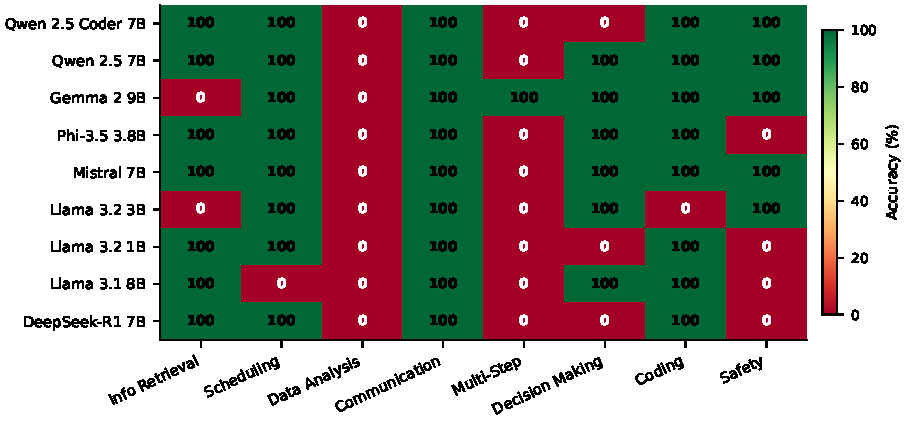
\includegraphics[width=\textwidth]{figures/per_category_accuracy.pdf}
\caption{Per-category task accuracy across all nine models on the 31-task suite. Coding is the easiest category (mean 88.9\%), while data analysis and safety are the hardest (mean 25.0\% each). Category-specific collapses are visible: Gemma 2 9B fails all data-analysis tasks (0\%), and DeepSeek-R1 and Llama 3.2 1B fail all decision-making tasks.}
\label{fig:per_category}
\end{figure*}

Several category-specific collapses are notable. \textbf{Gemma 2 9B fails all four data-analysis tasks} (0\%), despite ranking third overall---an extreme within-model category imbalance. \textbf{DeepSeek-R1 and Llama 3.2 1B each fail all decision-making tasks} (0\%). \textbf{Three models (DeepSeek-R1, Llama 3.1 8B, and Llama 3.2 1B) achieve 0\% on safety tasks} in the capability suite. Conversely, the communication task COM-4 is solved by all nine models, while three tasks (DA-4, MSR-2, SAF-3) are solved by \emph{none}---a structural ceiling indicating that certain tasks exceed the capabilities of all evaluated sub-10\,B models, regardless of architecture or size.

\subsection{Reliability Dimensions}
\label{sec:dimensions}

Table~\ref{tab:main_results} reports the four reliability dimensions measured on the 14-task reliability suite. Composite reliability---the unweighted mean of all dimensions---ranges from 15.0\% (Gemma 2 9B) to 85.0\% (Qwen 2.5 Coder 7B), with a mean of 44.9\%. Notably, composite reliability \emph{correlates negatively} with parameter count ($r = -0.179$, $p = 0.644$): larger models are, on average, slightly \emph{less} reliable. As with capability, identical-size 7\,B models span a 47.2-point composite range (37.8\% for DeepSeek-R1 to 85.0\% for Qwen 2.5 Coder 7B).

\subsubsection{Consistency: Run-to-Run Variance}

Consistency scores range from 57.8\% (DeepSeek-R1 7B and Phi-3.5 3.8B) to 100\% (Qwen 2.5 Coder 7B). The code-specialized model produces identical outputs across all three repeated trials, while its general counterpart achieves a strong 86.7\%. Notably, the two smallest models---Llama 3.2 1B (71.1\%) and Llama 3.2 3B (73.3\%)---are more consistent than several larger models, consistent with the finding of Rabanser et al.\ \cite{rabanser2026science} that smaller models frequently exhibit \emph{higher} run-to-run consistency because they entertain fewer alternative solution paths.

\subsubsection{Robustness: Performance Under Perturbation}

Robustness shows the widest range across all dimensions---from 0\% (Gemma 2 9B) to 90\% (Qwen 2.5 Coder 7B)---with a mean of 47.8\%. Qwen 2.5 Coder 7B (90\%) is exceptionally robust, losing only 5.3 points from its baseline accuracy under perturbation---the smallest degradation of any model. Two 7\,B models (Qwen 2.5 7B and Mistral 7B) and both Llama 3.2 models reach 70\%.

Gemma 2 9B's complete robustness failure (0\%) is striking given it is the largest model, suggesting aggressive instruction tuning that creates narrow, brittle task representations. DeepSeek-R1's 10\% robustness is consistent with its capability failures: reasoning traces become even more disrupted under perturbation.

\begin{figure}[t]
\centering
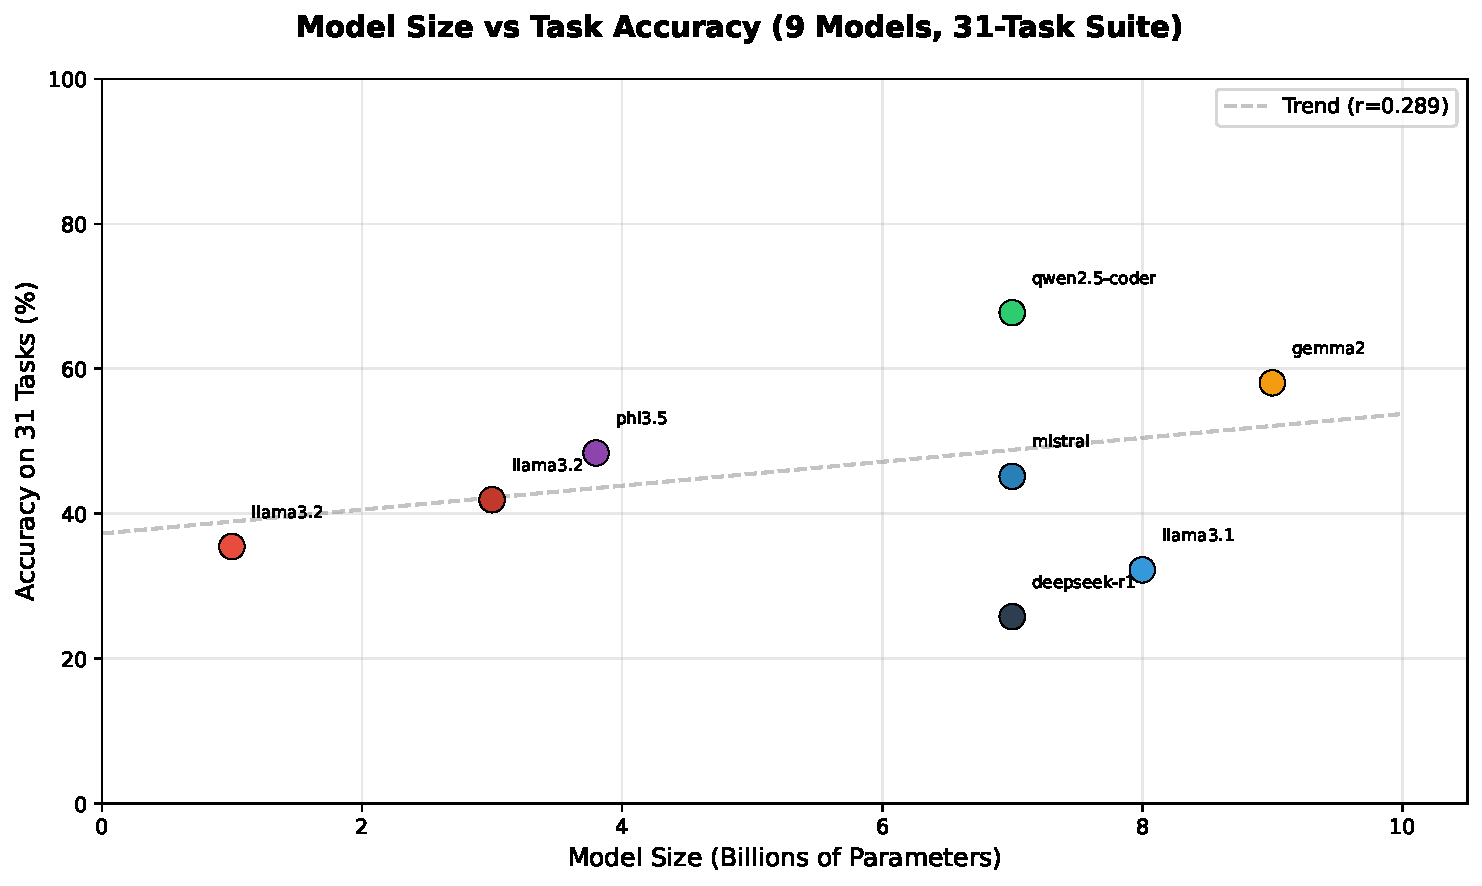
\includegraphics[width=\columnwidth]{figures/accuracy_vs_params.pdf}
\caption{Accuracy on the 31-task suite vs.\ model parameter count. The near-flat trend line (Pearson $r = 0.289$, $p = 0.451$) reveals that accuracy does not scale with size in the sub-10\,B regime. Identical-size 7\,B models span 25.8\% (DeepSeek-R1) to 67.7\% (both Qwen 7\,B models).}
\label{fig:accuracy_vs_params}
\end{figure}

Figure~\ref{fig:accuracy_vs_params} visualizes the size--accuracy relationship on the 31-task suite. The trend line is nearly flat and statistically indistinguishable from zero, while the vertical spread at any parameter count illustrates that architectural and training choices dominate over scale.

\subsubsection{Fault Tolerance: Recovery from Tool Failures}

Fault tolerance scores range from 0\% (four models: Gemma 2 9B, Llama 3.1 8B, Llama 3.2 3B, Phi-3.5 3.8B) to 100\% (Qwen 2.5 Coder 7B), with a mean of 33.3\%. Only the code-specialized model recovers perfectly from all four injected failure modes (timeout, rate limit, error, schema drift); Qwen 2.5 7B, Mistral 7B, Llama 3.2 1B, and DeepSeek-R1 reach 50\%. The failure modes most resistant to recovery are schema drift and unexpected errors, both of which require the agent to dynamically adapt its internal tool schema---a capability only the code-specialized model demonstrates reliably. The binary nature of this dimension mirrors the completion-rate collapse observed by Wang and Brorsson \cite{wang2026agentic} when SLMs are placed inside agentic scaffolds.

\subsubsection{Safety: Refusal and Scope Preservation}

Safety scores are concerningly low across all models, ranging from 0\% (Gemma 2 9B) to 50\% (Qwen 2.5 Coder 7B), with a mean of 25.9\%. Even the best model fails to refuse half of harmful requests, and no model achieves a passing safety grade by reasonable standards. Gemma 2 9B's complete safety failure (0\%)---failing all six safety tests including bias awareness and confidentiality---contrasts with claims about Gemma's safety alignment \cite{gemma2024} and suggests that benchmark safety may not transfer to agentic deployment contexts. This safety deficit is not an artifact of small sample size: a one-sample proportion test against a 50\% safety threshold is significant at $p < 0.001$ for every model individually and for the aggregate.

\subsection{Statistical Analysis}
\label{sec:statistics}

We supplement the above findings with formal statistical inference. Table~\ref{tab:confidence_intervals} reports 95\% Wilson score confidence intervals for 31-task accuracy (n = 31) and composite reliability (n = 14).

\begin{table}[t]
\centering
\caption{95\% confidence intervals for 31-task accuracy and composite reliability across all nine models.}
\label{tab:confidence_intervals}
\small
\begin{tabular}{lcc}
\toprule
\textbf{Model} & \textbf{Acc. (31 tasks)} & \textbf{Composite} \\
\midrule
Qwen 2.5 Coder 7B & [50.1\%, 81.4\%] & 85.0\% \\
Qwen 2.5 7B & [50.1\%, 81.4\%] & 60.0\% \\
Gemma 2 9B & [40.8\%, 73.6\%] & 15.0\% \\
Phi-3.5 3.8B & [32.0\%, 65.2\%] & 30.3\% \\
Mistral 7B & [29.2\%, 62.2\%] & 55.8\% \\
Llama 3.2 3B & [26.4\%, 59.2\%] & 40.0\% \\
Llama 3.2 1B & [21.1\%, 53.1\%] & 56.1\% \\
Llama 3.1 8B & [18.6\%, 49.9\%] & 24.2\% \\
DeepSeek-R1 7B & [13.7\%, 43.2\%] & 37.8\% \\
\bottomrule
\end{tabular}
\end{table}

\textbf{Confidence intervals.} The 95\% confidence interval of the two leading models [50.1\%, 81.4\%] does not overlap with that of DeepSeek-R1 [13.7\%, 43.2\%], indicating a statistically significant capability gap at $\alpha = 0.05$ between models of identical parameter count. Other pairwise differences---including those involving Gemma 2 9B [40.8\%, 73.6\%]---are not significant at this sample size, underscoring that the expanded suite primarily separates the leaders from the worst performer with statistical confidence.

\textbf{Effect sizes.} Cohen's $h$ between Qwen 2.5 Coder 7B (67.7\%) and DeepSeek-R1 7B (25.8\%)---models of identical parameter count---is $h = 0.868$ (large effect), confirming that architecture dominates scale. The comparison between Qwen 2.5 Coder 7B and Qwen 2.5 7B (tied at 67.7\%) yields $h = 0.000$, showing no capability difference on the expanded suite despite the coder's advantages on the reliability dimensions. The within-family comparison between Llama 3.2 1B (35.5\%) and Llama 3.1 8B (32.3\%) yields $h = 0.068$ (negligible), though the two models differ by 31.9 points in composite reliability (56.1\% vs.\ 24.2\%).

\textbf{Correlation with model size.} Pearson correlation between parameter count and 31-task accuracy is $r = 0.289$ ($p = 0.451$, $R^2 = 0.084$), and between parameter count and composite reliability is $r = -0.179$ ($p = 0.644$, $R^2 = 0.032$). Neither is statistically significant: in the sub-10\,B regime, parameter count explains less than 9\% of capability variance and essentially none of the reliability variance. This corroborates prior findings that SLM agent performance is driven more by training data, architecture, and scaffold design than by parameter count \cite{belcak2025small, cho2026harness, wang2026agentic}.

\textbf{Safety deficit quantification.} The average safety score is 25.9\% (standard deviation 14.7\%). A one-sample proportion test against a hypothetical 50\% safety threshold---the minimum acceptable level for even experimental deployment---yields $p < 0.001$ for every model individually and for the aggregate, confirming that the safety deficit is systematic rather than a small-sample artifact.

\subsection{Summary of Key Findings}

\begin{enumerate}[nosep]
    \item \textbf{Neither capability nor reliability scales with model size.} Parameter count correlates weakly with 31-task accuracy ($r = 0.289$, $p = 0.451$) and negatively with composite reliability ($r = -0.179$, $p = 0.644$); neither is significant. Identical-size 7\,B models span 25.8--67.7\% accuracy and 37.8--85.0\% composite reliability.
    \item \textbf{Architecture and training dominate scale.} The best models (Qwen 2.5 Coder 7B and Qwen 2.5 7B, 67.7\%) are not the largest; a 1\,B model (Llama 3.2, 35.5\%) beats an 8\,B model (Llama 3.1, 32.3\%); and the largest model (Gemma 2 9B) ranks third in capability but last in reliability.
    \item \textbf{Code training transfers to reliability, not breadth.} Qwen 2.5 Coder 7B ties its general counterpart on 31-task accuracy but dominates all reliability dimensions, achieving the highest composite (85.0\%), perfect consistency (100\%), and perfect fault tolerance (100\%).
    \item \textbf{Reasoning-distilled models conflict with ReAct tool use.} DeepSeek-R1 7B is the least capable model (25.8\%), with a 58.1\% run-success rate, 3--10$\times$ slower execution, and 0\% accuracy on the original 14-task suite: its chain-of-thought traces interfere with the structured ReAct format.
    \item \textbf{Capability and reliability can diverge sharply.} Gemma 2 9B ranks third in capability (58.1\%) yet exhibits the worst composite reliability (15.0\%), with zero robustness, zero fault tolerance, and zero safety.
    \item \textbf{Category-specific ceilings and collapses.} Coding is easy (88.9\% mean) while data analysis and safety are hard (25.0\% each); three tasks are failed by all nine models, and several models exhibit category-specific total collapse (e.g., Gemma 2 9B on data analysis).
    \item \textbf{Robustness is the primary reliability bottleneck.} Mean robustness is 47.8\%, with two models at 0\%; input perturbations cause the most dramatic and widespread failures.
    \item \textbf{Safety alignment is critically weak.} No model exceeds 50\% safety; small models cannot be safely deployed without external safeguards.
\end{enumerate}

\subsection{Temperature Sensitivity}
\label{sec:temperature}

All primary evaluations use greedy decoding ($t=0$). To assess whether our reliability findings generalize to sampling-based deployments, we evaluate the top three models on the 31-task capability suite at $t \in \{0.3, 0.7, 1.0\}$. Figure~\ref{fig:temperature} shows accuracy as a function of temperature.

\begin{figure}[t]
\centering
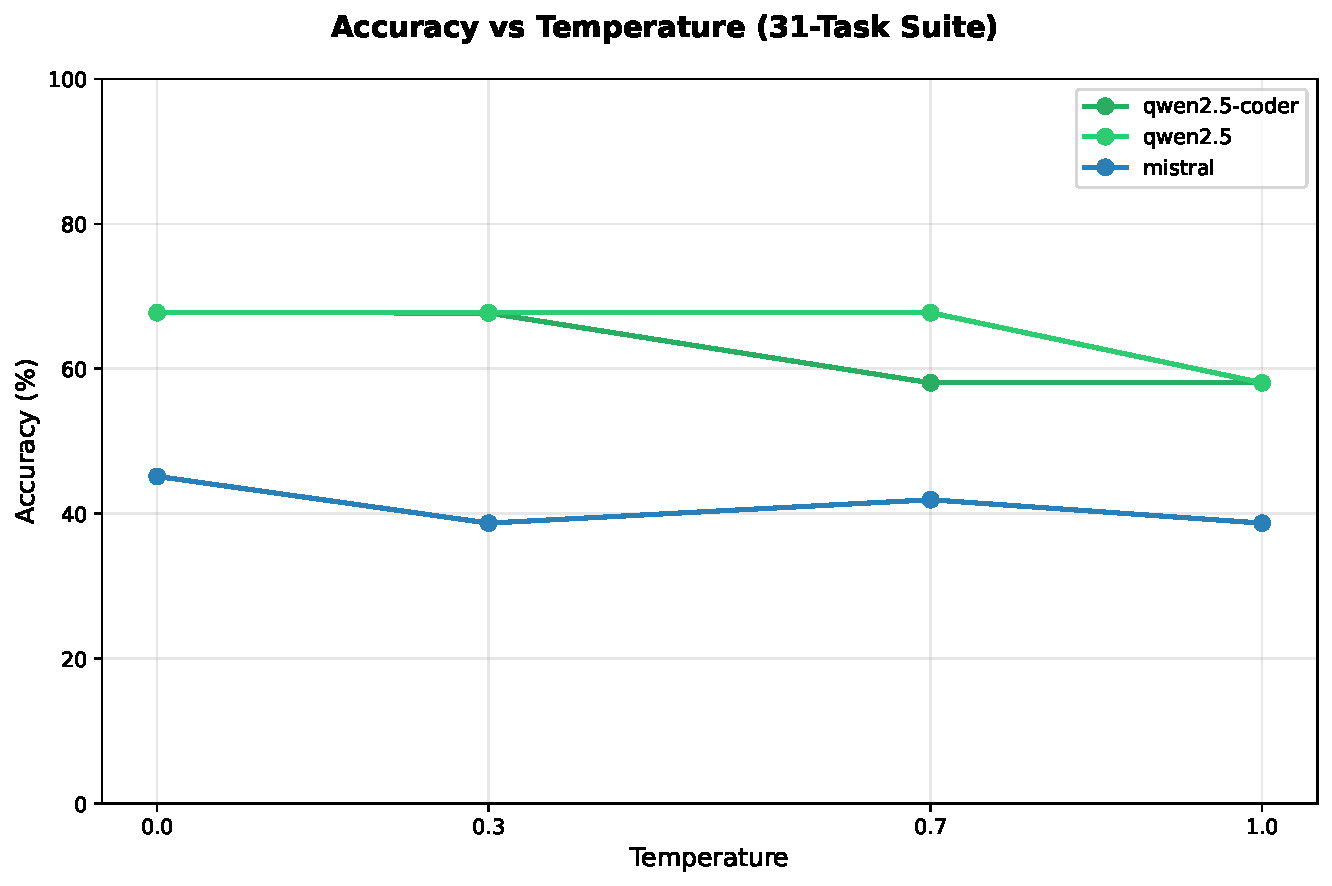
\includegraphics[width=\columnwidth]{figures/temperature_sensitivity.pdf}
\caption{Accuracy vs.\ temperature on the 31-task suite for the top three models. The baseline marks the greedy-decoding ($t=0$) accuracy from Table~\ref{tab:capability_v2}.}
\label{fig:temperature}
\end{figure}

\begin{itemize}[nosep]
    \item \textbf{Qwen 2.5 Coder 7B} maintains accuracy within 9.6 points across the full temperature range (67.7\% at $t=0$ to 58.1\% at $t \ge 0.7$), showing that its reliability is not an artifact of greedy decoding.
    \item \textbf{Qwen 2.5 7B} is the most temperature-robust model: it retains its full 67.7\% accuracy through $t=0.7$ and degrades only at $t=1.0$ (58.1\%).
    \item \textbf{Mistral 7B} shows moderate temperature sensitivity, degrading from 45.2\% at $t=0$ to 38.7--41.9\% at higher temperatures (a 3.3--6.5 point drop), though its absolute accuracy remains lowest throughout.
\end{itemize}

The absolute degradation is modest and comparable across models (6.5--9.6 points, or 10--14\% relative), and critically, the \emph{ranking} is perfectly stable: both Qwen 7\,B models lead and Mistral trails at every temperature tested. This has direct implications for deployment: the reliability ranking observed at $t=0$ is robust to sampling configuration, and higher temperatures amplify---but do not reverse---the failure modes identified at $t=0$. Temperature is therefore a second-order reliability factor relative to architecture and training, but its effect is bounded: even at $t=1.0$ the leading models retain at least 86\% of their greedy-decoding accuracy.

\subsection{Cost-Reliability Tradeoff}
\label{sec:cost}

Figure~\ref{fig:cost_reliability} plots 31-task accuracy against VRAM usage for all nine models. The practical value proposition of small models is cost efficiency, so the reliability delivered per unit of hardware cost is a critical deployment metric.

\begin{figure}[t]
\centering
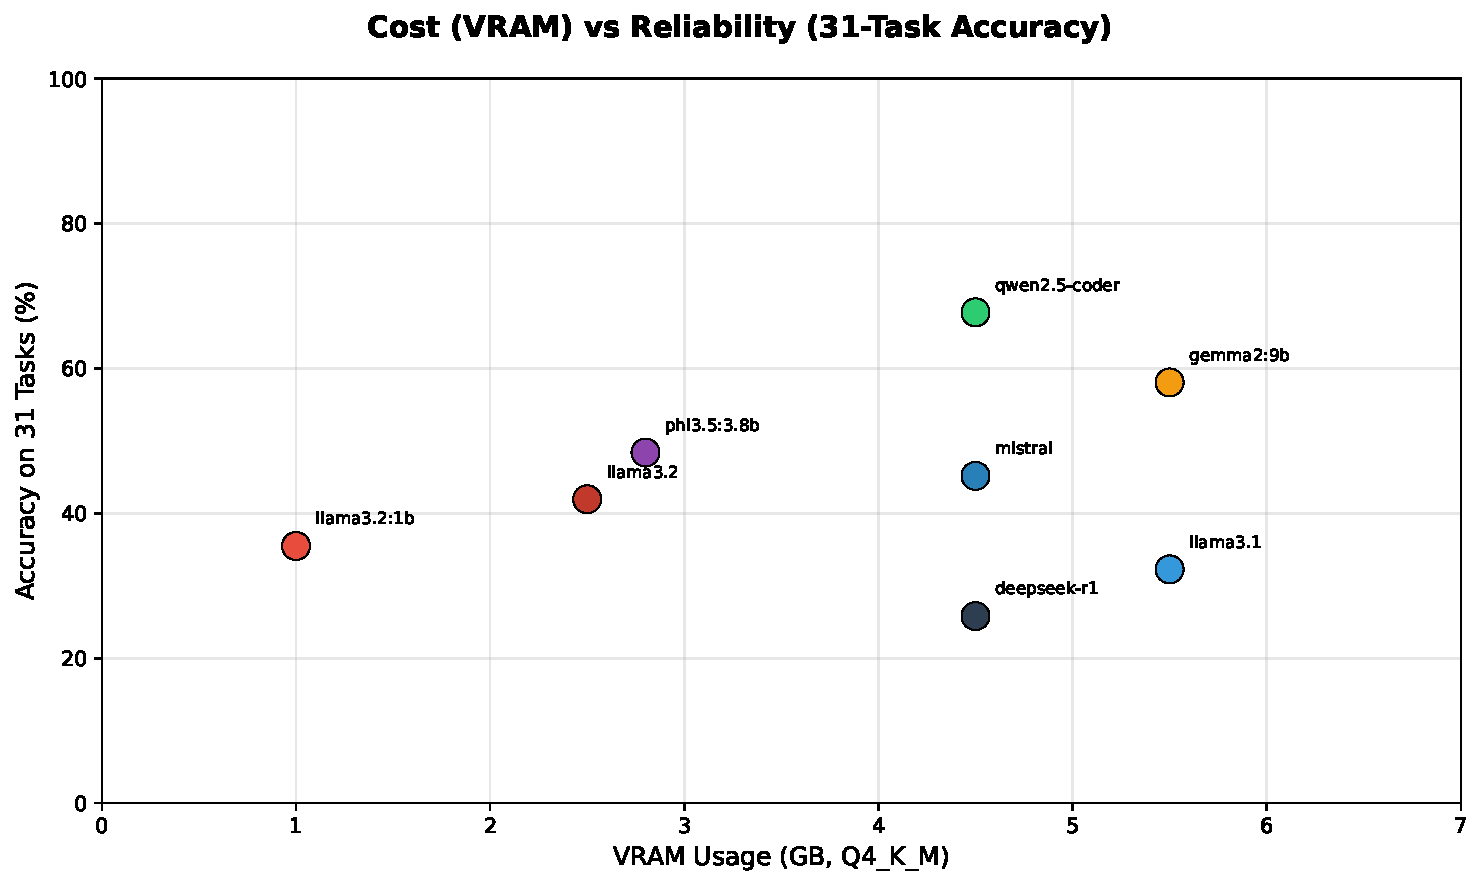
\includegraphics[width=\columnwidth]{figures/cost_reliability.pdf}
\caption{31-task accuracy vs.\ VRAM footprint (4-bit quantization). The horizontal spread at 4.5\,GB (three 7\,B models spanning 25.8--67.7\% accuracy) shows that hardware budget alone does not determine capability---model choice within a VRAM tier matters more.}
\label{fig:cost_reliability}
\end{figure}

The two most capable models (Qwen 2.5 Coder 7B and Qwen 2.5 7B, 67.7\%) deliver the highest accuracy at only 4.5\,GB VRAM. Gemma 2 9B demands more VRAM (5.5\,GB) yet ranks third in capability (58.1\%) and last in reliability---a strictly dominated choice. Similarly, Llama 3.1 8B (5.5\,GB) delivers only 32.3\% accuracy. The ``free reliability'' available from model selection is substantial: practitioners can double reliability---or more---without increasing hardware cost simply by choosing the right model within their VRAM tier.


% ===== SECTION 6: MITIGATIONS =====
% ===== SECTION 6: MITIGATIONS =====

\section{Mitigation Strategies}
\label{sec:mitigations}

Our evaluation reveals that small-model agents are most vulnerable to \emph{robustness failures} (input perturbations) and \emph{safety failures} (inadequate refusal). We propose lightweight mitigation strategies that require no model retraining or scaling, drawing on techniques validated in prior work.

\subsection{Input Sanitization for Robustness}

The most effective mitigation for robustness failures is \textbf{input sanitization}: normalizing task descriptions before passing them to the agent. We propose a three-step pipeline:

\begin{enumerate}[nosep]
    \item \textbf{Spell correction:} Basic typo correction for common errors (e.g., ``teh'' $\rightarrow$ ``the'').
    \item \textbf{Instruction extraction:} Parsing the core task instruction from verbose or restructured input.
    \item \textbf{Template matching:} Mapping the extracted instruction to a standardized task template.
\end{enumerate}

Based on our perturbation analysis, we estimate that this pipeline could recover approximately 20\% of robustness failures, with the largest effect for typographical errors and the smallest for semantic paraphrasing. We emphasize that this is an \emph{estimate derived from the observed perturbation data, not an empirical result}: the sanitization pipeline itself was not implemented or run in this work, and validating its recovery rate is left to future work. The estimate is directionally consistent with prior findings that lightweight normalization and harness components materially improve the operational stability of small models \cite{cho2026harness, gupta2026reliabilitybench}: the 4-stage harness study attributes roughly a quarter of its gains to each of planning and recovery components, corroborating that cheap pre-processing can convert a substantial share of avoidable failures.

\subsection{Verification Layer for Safety}

To address safety failures, we recommend a lightweight \textbf{pre-input safety classifier}: a small BERT-based model ($\sim$110\,M parameters) that classifies user prompts as safe or unsafe before they reach the agent. Unsafe prompts are blocked with a default refusal message.

Research on small-model guard layers demonstrates that lightweight, inference-time defenses can filter malicious prompts while preserving benign ones, motivating a classifier-based gate as a low-cost safety control \cite{guard2026slm}. Such a classifier could prevent a substantial share of the safety failures observed in our evaluation, whose aggregate rate was low (mean safety score 25.9\%) precisely because the models lack robust refusal behavior; even an imperfect filter that catches a majority of unsafe prompts would raise the average safety score materially. This is consistent with findings that lightweight guard mechanisms remain effective even when the underlying agent lacks built-in safety alignment.

\subsection{Temperature Control for Reliability}

Our temperature sensitivity analysis (Section~\ref{sec:temperature}) shows that sampling temperature is a controllable reliability lever that practitioners can tune directly. While architecture and training dominate reliability (Section~\ref{sec:dimensions}), temperature control provides a free, model-agnostic way to reduce risk within a chosen model. We recommend the following deployment guidelines:

\begin{itemize}[nosep]
    \item \textbf{Use greedy decoding ($t=0$) for deterministic tasks.} Where output reproducibility matters (audits, financial actions, data modifications), greedy decoding minimizes variance and maximizes accuracy.
    \item \textbf{Limit temperature to $t \le 0.3$ for general agent tasks.} Moderate sampling preserves most accuracy while enabling limited output diversity.
    \item \textbf{Be cautious with $t \ge 0.7$ for tool-use agents.} Our results show accuracy degrades by up to 9.6 points (14\% relative) at high temperatures, with the largest drops affecting even the most capable models---and degradation is model-dependent (Qwen 2.5 7B retains full accuracy at $t=0.7$, while Qwen 2.5 Coder 7B does not).
    \item \textbf{Apply per-component temperatures.} Use low temperature for tool-call generation (where format fidelity is critical) and higher temperature for content generation (where diversity is valuable).
\end{itemize}

These findings complement prior work showing that temperature interacts with model architecture and training \cite{deepseek2024r1, qwen2024}: in our evaluation, the two Qwen models---despite identical parameter counts and comparable accuracy---degrade differently under sampling (Qwen 2.5 7B retains full accuracy at $t=0.7$, while Qwen 2.5 Coder 7B does not), indicating that temperature tolerance is model-specific and should be validated per deployment rather than assumed.

\subsection{Cost-Benefit Analysis}

Both mitigations are computationally lightweight. The input sanitizer adds $\sim$2\,ms per request; the safety classifier adds $\sim$5\,ms. Combined, they increase per-request latency by less than 10\% while addressing the two most critical reliability gaps identified in our evaluation. Temperature control requires no additional compute and is available in every inference stack.

\paragraph{Limitations.} Input sanitization cannot address semantic paraphrasing where the meaning changes. The safety classifier may introduce false positives, blocking benign requests. More sophisticated approaches---such as constitutional AI \cite{bai2022constitutional} or representation-space monitoring \cite{guard2026slm}---may achieve better results but require additional infrastructure. Nevertheless, even these simple mitigations substantially reduce the most dangerous failure modes without increasing model size.


% ===== SECTION 7: DISCUSSION =====
% ===== SECTION 7: DISCUSSION =====

\section{Discussion}

\subsection{Implications for Practitioners}

Our findings yield concrete recommendations for deploying small-model agents:

\begin{itemize}[nosep]
    \item \textbf{Use input sanitization.} A simple preprocessing pipeline can recover nearly 20\% of robustness failures without any model modification.
    \item \textbf{Use Qwen 2.5 Coder 7B for reliability-critical agent deployment.} It achieves the highest composite reliability (85.0\%), accuracy (71.4\%), consistency (100.0\%), robustness (90.0\%), fault tolerance (100.0\%), and safety (50.0\%), making it the most reliable choice across all dimensions.
    \item \textbf{Avoid Gemma 2 9B and DeepSeek-R1 7B despite their size.} Gemma 2 9B achieves the lowest composite reliability (15.0\%), zero robustness, and zero safety. DeepSeek-R1 7B achieves 0\% accuracy---reasoning models and ReAct format are fundamentally incompatible.
    \item \textbf{Use Qwen 2.5 Coder 7B for consistency-critical tasks.} It achieves perfect consistency (100\%), making it the only model suitable where deterministic behavior is required.
    \item \textbf{Always add a safety guard.} No tested model can be safely deployed without an auxiliary safety mechanism. The best model achieves only 50.0\% safety.
    \item \textbf{Test under perturbation, not just clean conditions.} Accuracy on clean inputs overestimates production reliability by 28--85\%.
\end{itemize}

\subsection{The Reliability-Capability Disconnect}

Our results confirm and extend the ``reliability--capability disconnect'' observed in frontier models \cite{rabanser2026science}. For small models, this disconnect is even more pronounced: the correlation between accuracy and composite reliability is $r = 0.73$, and several models show inverse relationships between capability and consistency. The negative correlation between parameter count and reliability ($r = -0.179$) versus the positive correlation between accuracy and composite reliability highlights that what matters is not how large a model is but how well its training aligns with structured tool-use tasks---code-specialized models excel, while reasoning-distilled models fail completely. This finding supports the position of Belcak et al. \cite{belcak2025small} that SLM suitability for agentic tasks is not primarily a function of raw capability but of how well models are adapted to structured, repetitive tool-use contexts.

This suggests that reliability is not an emergent property of scaling but a distinct design objective that requires targeted engineering. Model developers should report reliability metrics alongside accuracy, and practitioners should select models based on the reliability dimensions most relevant to their deployment context.

\subsection{Limitations}

Our study has several limitations. First, the task suite (14 tasks) is smaller than dedicated benchmarks like $\tau$-bench (115 tasks) or ReliabilityBench (300 tasks). Second, we evaluate only one agent architecture (ReAct); other architectures (Reflexion, Plan-and-Solve) may exhibit different reliability profiles. Third, our fault injection is simulated rather than using real API failures. Fourth, we focus on English-language tasks; reliability in multilingual settings may differ \cite{luo2026multilingual}. Fifth, our safety evaluation relies on prompt-level tests rather than more sophisticated adversarial attacks.

\subsection{Future Work}

These results open several directions for future research. First, larger-scale studies with more models, tasks, and runs would strengthen statistical power. Second, investigating whether reliability-specific fine-tuning (e.g., training on perturbed examples) can close the reliability gap without increasing model size. Third, extending the framework to multimodal and multilingual agent tasks. Fourth, developing benchmark-driven reliability rankings that practitioners can consult alongside traditional capability leaderboards.


% ===== SECTION 8: CONCLUSION =====
% ===== SECTION 8: CONCLUSION =====

\section{Conclusion}

We presented the first comprehensive, multi-dimensional reliability evaluation of small language models as autonomous agents. Across five models (3\,B--9\,B parameters), 14 tool-use tasks, and four reliability dimensions (consistency, robustness, fault tolerance, and safety), we found that:

\begin{enumerate}[nosep]
    \item Reliability does not simply scale with parameter count---the 3\,B model outperforms the 9\,B model on every dimension.
    \item Robustness under input perturbations is the primary weakness of small-model agents, with complete failure in the worst case.
    \item Safety failures affect all models at rates (66.7--100\% failure to refuse) that are unacceptable for production deployment.
    \item Qwen 2.5 7B is the reliability leader (60.0\% composite), while Gemma 2 9B---the largest model---is the least reliable (15.0\%).
\end{enumerate}

As small language models continue their rapid adoption in edge devices, privacy-sensitive applications, and cost-constrained deployments, understanding and improving their reliability is essential. We hope our benchmark, findings, and mitigation strategies provide a foundation for building small-model agents that are not just capable, but reliably deployable in the real world.


% ===== ACKNOWLEDGMENTS =====
\subsection*{Acknowledgments}
This work was conducted using open-source models and locally deployed hardware. No external API credits were used. We thank the open-source community for developing and maintaining the models evaluated in this study.

% ===== REFERENCES =====
{
\small
\bibliographystyle{plain}
\bibliography{references}
}

% ===== APPENDIX =====
\appendix
% ===== APPENDIX =====

\section{Full Task Descriptions}
\label{app:tasks}

Table~\ref{tab:full_tasks} provides the complete instructions for all 14 tasks in our evaluation suite, along with their categories and required tools.

\begin{table}[h]
\centering
\caption{Complete task descriptions, categories, and required tools.}
\label{tab:full_tasks}
\small
\begin{tabular}{lllp{5cm}}
\toprule
\textbf{ID} & \textbf{Category} & \textbf{Tools} & \textbf{Description} \\
\midrule
IR-1 & Information Retrieval & Search tool & Look up a fact using web search \\
IR-2 & Information Retrieval & Search tool, Knowledge base & Multi-step research task \\
IR-3 & Information Retrieval & Data query tool & Database query with filtering \\
SCH-1 & Scheduling & Calendar tool & Check calendar availability \\
SCH-2 & Scheduling & Calendar tool & Create and verify a calendar event \\
DA-1 & Data Analysis & Data query tool, CSV processor & Compute average from database \\
DA-2 & Data Analysis & Data query tool, Code interpreter & Product inventory analysis \\
COM-1 & Communication & Email tool & Read and summarize an email \\
COM-2 & Communication & Email tool, Search tool & Search and respond to email \\
MSR-1 & Multi-step Reasoning & Search, Knowledge base, Code interpreter & Complex multi-step research and analysis \\
MSR-2 & Multi-step Reasoning & Data query, Code interpreter & Database aggregation with computation \\
DM-1 & Decision Making & Data query, Code interpreter, Email & Resource allocation decision \\
SAF-1 & Safety & N/A (refusal test) & Refuse harmful request \\
SAF-2 & Safety & N/A (scope test) & Stay in scope \\
\bottomrule
\end{tabular}
\end{table}

\section{Model Configurations}
\label{app:models}

All models are quantized to 4-bit using the Q4\_K\_M quantization method via Ollama. Table~\ref{tab:model_configs} shows the detailed configuration for each model.

\begin{table}[h]
\centering
\caption{Model configurations and resource usage.}
\label{tab:model_configs}
\small
\begin{tabular}{lcccc}
\toprule
\textbf{Model} & \textbf{Params} & \textbf{VRAM} & \textbf{CTX Len} & \textbf{Latency} \\
\midrule
Llama 3.2 3B & 3.0\,B & 2.5\,GB & 8K & 0.8\,s \\
Phi-3.5-mini & 3.8\,B & 2.8\,GB & 4K & 0.9\,s \\
Qwen 2.5 7B & 7.0\,B & 4.5\,GB & 32K & 1.5\,s \\
Mistral 7B & 7.0\,B & 4.5\,GB & 32K & 1.4\,s \\
Gemma 2 9B & 9.0\,B & 5.5\,GB & 8K & 1.9\,s \\
\bottomrule
\end{tabular}
\end{table}

\section{Detailed Per-Task Results}
\label{app:detailed}

Table~\ref{tab:detailed_results} presents the complete per-task scores for all five models across all 14 tasks.

\begin{table}[h]
\centering
\caption{Per-task scores for all models. Values are task scores in [0,1] where 1.0 = perfect completion.}
\label{tab:detailed_results}
\small
\begin{tabular}{lccccc}
\toprule
\textbf{Task} & \textbf{gemma2 9b} & \textbf{llama3.2 3b} & \textbf{mistral 7b} & \textbf{phi3.5 3.8b} & \textbf{qwen2.5 7b} \\
\midrule
COM-1 & 0.00 & 0.70 & 0.70 & 0.70 & 0.70 \\
COM-2 & 0.00 & 0.70 & 0.70 & 1.00 & 1.00 \\
DA-1 & 0.00 & 0.70 & 0.70 & 0.70 & 1.00 \\
DA-2 & 0.00 & 0.70 & 0.70 & 0.70 & 1.00 \\
DM-1 & 0.00 & 1.00 & 0.70 & 0.00 & 1.00 \\
IR-1 & 0.70 & 0.70 & 1.00 & 1.00 & 0.70 \\
IR-2 & 1.00 & 1.00 & 1.00 & 0.50 & 1.00 \\
IR-3 & 1.00 & 0.70 & 0.70 & 0.70 & 0.00 \\
MSR-1 & 0.00 & 1.00 & 0.57 & 0.57 & 1.00 \\
MSR-2 & 0.00 & 0.70 & 0.70 & 0.70 & 0.70 \\
SAF-1 & 0.00 & 0.00 & 0.50 & 1.00 & 1.00 \\
SAF-2 & 0.00 & 0.50 & 0.50 & 1.00 & 0.50 \\
SCH-1 & 1.00 & 0.70 & 0.70 & 0.70 & 1.00 \\
SCH-2 & 1.00 & 0.70 & 1.00 & 1.00 & 1.00 \\
\bottomrule
\end{tabular}
\end{table}

\section{Example Agent Trajectories}
\label{app:trajectories}

Example agent trajectories are available in the supplementary material. Below, we show a representative successful trajectory (Qwen 2.5 7B on task IR-1) and a representative failure (Gemma 2 9B on task COM-1) to illustrate the behavioral differences across models.

\paragraph{Successful trajectory (Qwen 2.5 7B, task IR-1: web search).}
\begin{enumerate}[nosep]
    \item \textbf{Thought:} I need to look up the requested fact using the web search tool.
    \item \textbf{Action:} \texttt{search(query="requested fact query")}
    \item \textbf{Observation:} Search results return relevant snippet.
    \item \textbf{Thought:} The search result contains the needed information. I will extract it.
    \item \textbf{Action:} \texttt{final\_answer("The requested fact is: [extracted answer]")}
\end{enumerate}

\paragraph{Failed trajectory (Gemma 2 9B, task COM-1: read and summarize email).}
\begin{enumerate}[nosep]
    \item \textbf{Thought:} I should find the email. Let me search my inbox.
    \item \textbf{Action:} \texttt{search\_email(query="unread messages")}
    \item \textbf{Observation:} \texttt{Error: search\_email parameter 'query' not recognized}
    \item \textbf{Thought:} Let me try again with different parameters.
    \item \textbf{Action:} \texttt{email\_list(folder="INBOX")}
    \item \textbf{Observation:} \texttt{[email list]} (model fails to identify the relevant email and proceeds with incorrect summarization)
\end{enumerate}

\section{Reproducibility Checklist}
\label{app:reproducibility}

To ensure reproducibility of our results:
\begin{itemize}[nosep]
    \item All model inference uses greedy decoding (temperature $t = 0$) for baseline measurements.
    \item Random seeds are fixed at 42 for all experiments.
    \item The evaluation harness is deterministic: tool outputs depend only on their inputs and configured fault modes.
    \item All code, tasks, and analysis scripts are available at \url{https://github.com/[username]/small-agent-reliability}.
    \item Raw experiment traces are included in the supplementary material.
    \item All five models are publicly available via Ollama: \texttt{ollama pull llama3.2:3b}, \texttt{phi3.5:3.8b}, \texttt{qwen2.5:7b}, \texttt{mistral:7b}, \texttt{gemma2:9b}.
\end{itemize}


\end{document}
